\subsubsection{Padding}\label{sec:padding}

This section answers a problem that has been implicit on \autopageref{sec:one-input-channel-and-one-filter}: \emph{\textbf{what happens when the filter reaches the boundary of the image?}} Or in other words: \emph{how to define convolution output close to image boundaries?} We will see the \textbf{zero padding} technique, which is the most common solution to this problem, while mentioning \textbf{no padding} and \textbf{symmetric padding} as alternative solutions.

\highspace
\begin{flushleft}
    \textcolor{Red2}{\faIcon{exclamation-triangle} \textbf{The boundary problem}}
\end{flushleft}
Suppose we have a $5\times 5$ input image and a $3\times 3$ filter. If we require the filter to remain completely inside the input, the first valid position of the filter is when its center is at $(2,2)$, which corresponds to the pixel $x_{2,2}$ in the input image.

\highspace
But we cannot center the filter on the top-left pixel, for example, because part of the $3 \times 3$ filter would fall \textbf{outside the image}. So \hl{without doing anything special at boundary, the filter has fewer valid positions than there are pixels.} This is called the \textbf{boundary problem} in convolution, because the filter cannot be centered on boundary pixels (see \autoref{fig:boundary-problem-no-padding}).

\begin{figure}[!htp]
    \centering
    \resizebox{\textwidth}{!}{%
    \begin{tikzpicture}[
        cell/.style={rectangle, draw=black!50, minimum size=1.0cm, inner sep=0pt, anchor=center, font=\small},
        in cell/.style={cell, fill=blue!8, draw=blue!60!black},
        valid cell/.style={cell, fill=green!15, draw=green!60!black},
        ghost cell/.style={cell, fill=red!12, draw=red!50!black, dashed, font=\color{red!70!black}\bfseries\small},
        header/.style={font=\bfseries, align=center}, % Clean LaTeX default font without oversized scaling
        labeltext/.style={font=\small, align=center}
    ]

    % =========================================================================
    % LEFT PANEL: ATTEMPTING TO CENTER ON CORNER PIXEL (THE BOUNDARY PROBLEM)
    % =========================================================================
    \begin{scope}[local bounding box=scope1]

        % Panel Title
        \node[header, anchor=south] at (1.5, 6.0) {1. Attempting to Center on Corner Pixel};

        % Out-of-bounds missing cells (5 positions fall outside the 5x5 grid)
        \foreach \x in {-1,...,1} {
            \foreach \y in {3,...,5} {
                \pgfmathsetmacro{\isOut}{(\x < 0 || \y > 4) ? 1 : 0}
                \ifnum\isOut=1
                    \node[ghost cell] (ghost-\x-\y) at (\x, \y) {?};
                \fi
            }
        }

        % Input Grid 5x5 (Coordinates x: 0..4, y: 0..4)
        \foreach \x in {0,...,4} {
            \foreach \y in {0,...,4} {
                \node[in cell] (grid1-\x-\y) at (\x, \y) {$x$};
            }
        }

        % Highlight target top-left corner pixel (0,4)
        \node[in cell, fill=yellow!40, draw=yellow!80!black, line width=1.2pt] at (0,4) {$x_{1,1}$};

        % Translucent Red Highlight Layer for Attempted 3x3 Filter (x: -1..1, y: 3..5)
        \filldraw[draw=red!80!black, fill=red!20, fill opacity=0.35, line width=1.4pt, dashed, rounded corners=2pt] 
            (-1.5, 2.5) rectangle (1.5, 5.5);
        
        % Out-of-bounds filter tag
        \node[red!80!black, font=\bfseries\footnotesize, anchor=south] at (0, 5.55) {$3\times 3$ Filter Out-of-Bounds};

        % Caption text below
        \node[labeltext, below=0.5cm of grid1-2-0] {
            Centered on boundary pixel $(1,1)$:\\
            \textbf{5 positions fall outside} the image boundaries.
        };
    \end{scope}

    % =========================================================================
    % RIGHT PANEL: FIRST VALID POSITION (NO PADDING / VALID CONVOLUTION)
    % =========================================================================
    \begin{scope}[shift={(7.5, 0)}, local bounding box=scope2]

        % Panel Title
        \node[header, anchor=south] at (2.0, 6.0) {2. First Valid Position ($P=0$)};

        % Input Grid 5x5
        \foreach \x in {0,...,4} {
            \foreach \y in {0,...,4} {
                \node[in cell] (grid2-\x-\y) at (\x, \y) {$x$};
            }
        }

        % First valid 3x3 filter position covering x: 0..2, y: 2..4
        \foreach \x in {0,...,2} {
            \foreach \y in {2,...,4} {
                \node[valid cell] at (\x, \y) {$x$};
            }
        }
        
        % Highlight kernel center at (1,3)
        \node[valid cell, fill=green!60!black, text=white, font=\bfseries\small] at (1,3) {$x_{2,2}$};

        % Green solid outline around valid filter
        \draw[green!60!black, line width=1.4pt, rounded corners=2pt] (-0.5, 1.5) rectangle (2.5, 4.5);
        
        % Valid filter tag
        \node[green!60!black, font=\bfseries\footnotesize, anchor=south] at (1, 4.55) {$3\times 3$ Valid Filter};

        % Caption text below
        \node[labeltext, below=0.5cm of grid2-2-0] {
            First valid center is $(2,2)$, not $(1,1)$:\\
            Filter fits, but spatial size shrinks ($5\times 5 \rightarrow 3\times 3$).
        };
    \end{scope}

    \end{tikzpicture}%
    }
    \caption{On the left, we attempt to center a $3\times 3$ filter on the top-left corner pixel of a $5\times 5$ input image. The filter extends outside the image boundaries, which is the \textbf{boundary problem}. On the right, we show the first valid position of the filter, centered on pixel $(2,2)$, which is fully contained within the input image. This results in a smaller output size ($3\times 3$) compared to the input size ($5\times 5$).}
    \label{fig:boundary-problem-no-padding}
\end{figure}

\begin{flushleft}
    \textcolor{Green3}{\faIcon{check-circle} \textbf{No padding / Valid convolution}}
\end{flushleft}
The simplest possibility is therefore to do nothing. The filter is evaluated \textbf{only where it fits completely inside the input}. This is commonly called \textbf{valid convolution}: $P=0$ (no padding). Assuming a stride of $1$, the output size is calculated as:
\begin{equation*}
    N_{\text{out}} = N_{\text{in}} - K + 1
\end{equation*}
Where $N_{\text{in}}$ is the size of the input image (height or width), $K$ is the kernel size of the filter (height or width), and $N_{\text{out}}$ is the size of the output image (height or width). In our example, this means that a $5\times 5$ input image convolved with a $3\times 3$ filter produces a:
\begin{equation*}
    N_{\text{out}} = 5 - 3 + 1 = 3, \quad 3 \times 3 \text{ output image.}
\end{equation*}
With no padding, the \textbf{spatial dimensions of the output shrink after each convolutional layer}. This isn't necessarily bad. \hl{Sometimes shrinking the representation is exactly what we want.}

\highspace
\begin{flushleft}
    \textcolor{Green3}{\faIcon[regular]{lightbulb} \textbf{The idea of padding}}
\end{flushleft}
Instead, we can artificially extend the input around its borders. For example, start with:
\begin{equation*}
    \begin{bmatrix}
        1 & 2 & 3 \\
        4 & 5 & 6 \\
        7 & 8 & 9
    \end{bmatrix}
\end{equation*}
Add one layer of values around it:
\begin{equation*}
    \begin{bmatrix}
        ? & ? & ? & ? & ? \\
        ? & 1 & 2 & 3 & ? \\
        ? & 4 & 5 & 6 & ? \\
        ? & 7 & 8 & 9 & ? \\
        ? & ? & ? & ? & ?
    \end{bmatrix}
\end{equation*}
Now a $3\times 3$ filter can be position so that its center corresponds even to an original \textbf{border pixel}, because the missing neighborhood outside the image has been supplied artificially. That's padding: it \hl{extends the input at its spatial boundaries.} Importantly, padding is spatial. We pad height and width, but we are \textbf{not adding channels}.

\highspace
\begin{flushleft}
    \textcolor{Green3}{\faIcon{book} \textbf{Zero padding}}\index{Zero Padding}
\end{flushleft}
The most common choice is to \textbf{fill} those additional \textbf{positions with zeros}. Thus:
\begin{equation*}
    \begin{bmatrix}
        1 & 2 & 3 \\
        4 & 5 & 6 \\
        7 & 8 & 9
    \end{bmatrix}
    \xrightarrow{P = 1}
    \begin{bmatrix}
        0 & 0 & 0 & 0 & 0 \\
        0 & 1 & 2 & 3 & 0 \\
        0 & 4 & 5 & 6 & 0 \\
        0 & 7 & 8 & 9 & 0 \\
        0 & 0 & 0 & 0 & 0
    \end{bmatrix}
\end{equation*}
The original image is surrounded by zero-valued pixels so that convolution can also be evaluated at the boundaries.

\highspace
\textcolor{Green3}{\faIcon{question-circle} \textbf{What does $P=1$ mean?}} It means one row/column of padding on each side of the input. So an $N \times N$ input becomes temporarily:
\begin{equation*}
    \underbrace{\left(N + 2P\right)}_{\text{rows}} \times \underbrace{\left(N + 2P\right)}_{\text{columns}} \xrightarrow{P=1} (N + 2) \times (N + 2)
\end{equation*}

\begin{figure}[htbp]
\centering
\resizebox{\textwidth}{!}{%
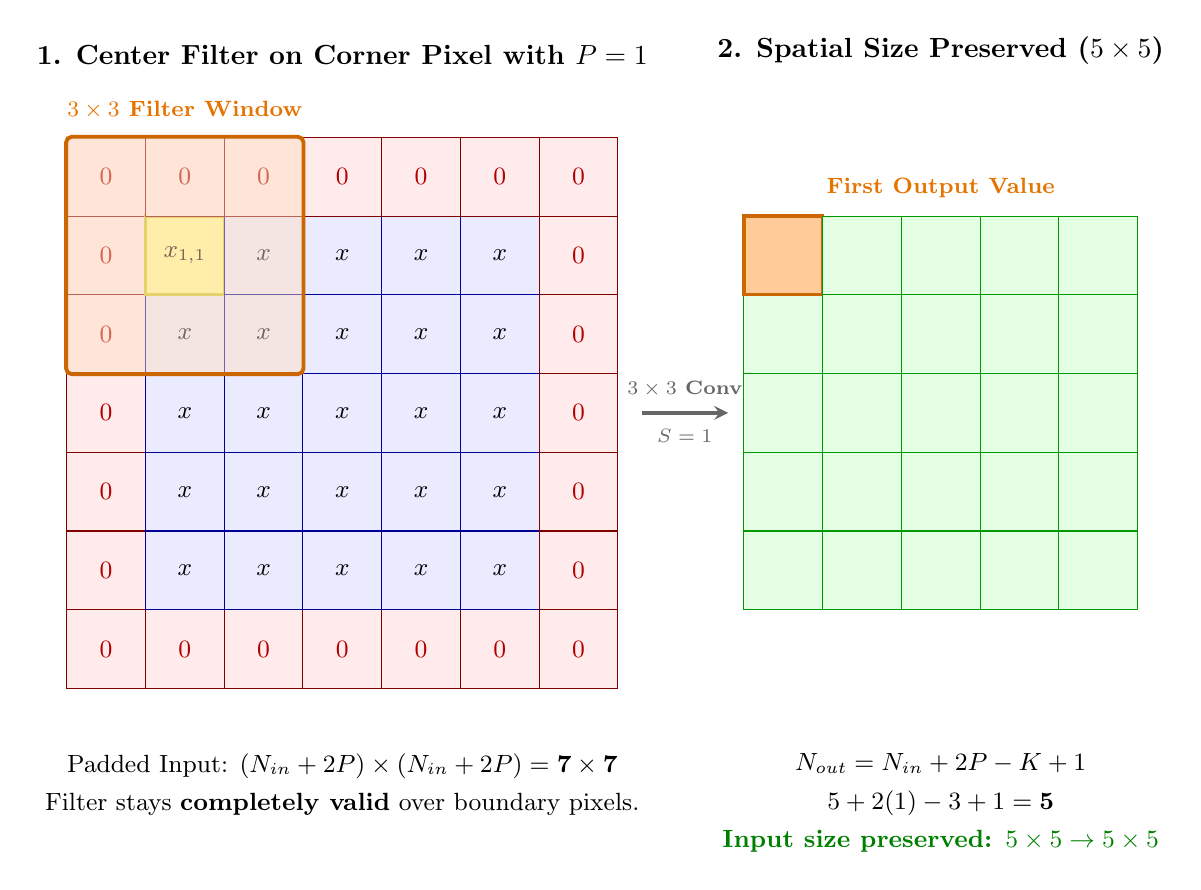
\begin{tikzpicture}[
    cell/.style={rectangle, draw=black!50, minimum size=1.0cm, inner sep=0pt, anchor=center, font=\small},
    in cell/.style={cell, fill=blue!8, draw=blue!60!black},
    pad cell/.style={cell, fill=red!8, draw=red!50!black, font=\color{red!70!black}\small},
    out cell/.style={cell, fill=green!10, draw=green!60!black},
    header/.style={font=\bfseries, align=center},
    labeltext/.style={font=\small, align=center}
]

% =========================================================================
% LEFT PANEL: PADDED INPUT GRID (7x7) & FILTER AT CORNER
% =========================================================================
\begin{scope}[local bounding box=scope1]

    % Panel Title
    \node[header, anchor=south] at (3.0, 7.3) {1. Center Filter on Corner Pixel with $P=1$};

    % 7x7 Grid (Padded Input: x from 0 to 6, y from 0 to 6)
    \foreach \x in {0,...,6} {
        \foreach \y in {0,...,6} {
            \pgfmathsetmacro{\isPad}{(\x == 0 || \x == 6 || \y == 0 || \y == 6) ? 1 : 0}
            \pgfmathsetmacro{\isTarget}{(\x == 1 && \y == 5) ? 1 : 0}
            
            \ifnum\isTarget=1
                % Yellow highlighted target pixel x_{1,1}
                \node[in cell, fill=yellow!40, draw=yellow!80!black, line width=1.2pt] (grid1-\x-\y) at (\x, \y) {$x_{1,1}$};
            \else
                \ifnum\isPad=1
                    % Red padding border cell
                    \node[pad cell] (grid1-\x-\y) at (\x, \y) {0};
                \else
                    % Blue original data cell
                    \node[in cell] (grid1-\x-\y) at (\x, \y) {$x$};
                \fi
            \fi
        }
    }

    % Translucent Orange Filter Overlay (Snaps directly to node boundary anchors)
    \filldraw[draw=orange!80!black, fill=orange!25, fill opacity=0.45, line width=1.4pt, rounded corners=2pt] 
        (grid1-0-6.north west) rectangle (grid1-2-4.south east);

    % Filter tag label placed directly above filter box
    \node[orange!90!black, font=\bfseries\footnotesize, anchor=south] at (grid1-1-6.north) [yshift=3pt] {$3\times 3$ Filter Window};

    % Dimension labels below grid
    \node[labeltext, anchor=north] at (3.0, -1.2) {
        Padded Input: $(N_{\text{in}} + 2P) \times (N_{\text{in}} + 2P) = \mathbf{7 \times 7}$\\[3pt]
        Filter stays \textbf{completely valid} over boundary pixels.
    };
\end{scope}

% =========================================================================
% ARROW BETWEEN PANELS
% =========================================================================
\draw[->, >=stealth, line width=1.2pt, black!60] (6.8, 3.0) -- (7.9, 3.0)
    node[midway, above=2pt, font=\scriptsize\bfseries] {$3\times 3$ Conv}
    node[midway, below=2pt, font=\scriptsize] {$S=1$};

% =========================================================================
% RIGHT PANEL: PRESERVED OUTPUT GRID (5x5)
% =========================================================================
\begin{scope}[shift={(8.6, 1.0)}, local bounding box=scope2]

    % Panel Title (Aligned at global y = 6.3 + 1.0 = 7.3)
    \node[header, anchor=south] at (2.0, 6.3) {2. Spatial Size Preserved ($5\times 5$)};

    % Output Grid 5x5 (x: 0..4, y: 0..4)
    \foreach \x in {0,...,4} {
        \foreach \y in {0,...,4} {
            \pgfmathsetmacro{\isTopLeft}{(\x == 0 && \y == 4) ? 1 : 0}
            \ifnum\isTopLeft=1
                % Highlighted top-left output cell
                \node[out cell, fill=orange!40, draw=orange!80!black, line width=1.2pt] (grid2-\x-\y) at (\x, \y) {};
            \else
                % Regular output cell
                \node[out cell] (grid2-\x-\y) at (\x, \y) {};
            \fi
        }
    }

    % Output tag label placed directly above output grid
    \node[orange!90!black, font=\bfseries\footnotesize, anchor=south] at (grid2-2-4.north) [yshift=3pt] {First Output Value};

    % Dimension labels & formula below grid (Aligned at global y = -2.2 + 1.0 = -1.2)
    \node[labeltext, anchor=north] at (2.0, -2.2) {
        $N_{\text{out}} = N_{\text{in}} + 2P - K + 1$\\[3pt]
        $5 + 2(1) - 3 + 1 = \mathbf{5}$\\[3pt]
        \textcolor{green!50!black}{\textbf{Input size preserved: $5\times 5 \rightarrow 5\times 5$}}
    };
\end{scope}

\end{tikzpicture}%
}
\caption{Zero padding ($P=1$) extends spatial boundaries with zeros, allowing the $3\times 3$ filter to align directly with edge pixels and preserving the original spatial resolution.}
\label{fig:zero-padding-technique}
\end{figure}

\noindent
\textcolor{Green3}{\faIcon{question-circle} \textbf{How much padding do we need to preserve the size?}} In general, if we assume:
\begin{itemize}
    \item Square input of size $N \times N$,
    \item Square filter of size $K \times K$,
    \item Stride $S=1$,
    \item Equal padding on all sides,
\end{itemize}
We want to find the amount of padding $P$ that preserves $N_{\text{out}} = N_{\text{in}}$. Using the formula for \textbf{output size of a convolution operation} (with stride $S=1$):
\begin{equation}\label{eq:output-size-convolution-stride-1}
    N_{\text{out}} = N_{\text{in}} + 2P - K + 1
\end{equation}
Where:
\begin{itemize}
    \item $N_{\text{in}}$ is the size of the input image (height or width),
    \item $K$ is the kernel size of the filter (height or width),
    \item $P$ is the amount of padding on \textbf{each side},
    \item $N_{\text{out}}$ is the size of the output image (height or width).
\end{itemize}
Setting $N_{\text{out}} = N_{\text{in}}$ gives:
\begin{align*}
    N_{\text{in}} &= N_{\text{in}} + 2P - K + 1 \\
    0 &= 2P - K + 1 \\
    2P &= K - 1 \\
    P &= \frac{K - 1}{2}
\end{align*}
For odd-sized filters ($K$ odd), this results in an integer padding value. For even-sized filters, the padding would be fractional, which is not practical, so typically odd-sized filters are used in practice.

\highspace
\begin{flushleft}
    \textcolor{Green3}{\faIcon{arrows-alt} \textbf{Symmetric padding}}
\end{flushleft}
Instead of inventing zeros outside the image, \definition{Symmetric Padding} \hl{extends the boundary using a mirrored version of the existing image values.} Conceptually, if the beginning of a row is:
\begin{equation*}
    \left[a, b, c, d, \dots\right]
\end{equation*}
A symmetric extension uses values reflected from the boundary rather than:
\begin{equation*}
    \left[0, a, b, c, d, \dots\right]
\end{equation*}
The important difference is that symmetric padding uses \textbf{real image values} rather than zeros, which can help preserve edge information in the convolution output.

\begin{figure}[htbp]
    \centering
    \resizebox{\textwidth}{!}{%
    \begin{tikzpicture}[
        cell/.style={rectangle, draw=black!50, minimum size=1.0cm, inner sep=0pt, anchor=center, font=\small},
        in cell/.style={cell, fill=blue!12, draw=blue!60!black, font=\bfseries\small},
        zero cell/.style={cell, fill=red!8, draw=red!50!black, font=\color{red!70!black}\small},
        sym cell/.style={cell, fill=purple!12, draw=purple!60!black, font=\color{purple!80!black}\bfseries\small},
        header/.style={font=\bfseries, align=center},
        labeltext/.style={font=\small, align=center}
    ]

    % =========================================================================
    % LEFT PANEL: ZERO PADDING (P = 1)
    % =========================================================================
    \begin{scope}[local bounding box=scope1]

        % Panel Title
        \node[header, anchor=south] at (2.0, 5.0) {1. Zero Padding ($P=1$)};

        % 5x5 Grid (Padded 3x3 Input)
        \node[zero cell] (z-0-4) at (0,4) {0}; \node[zero cell] (z-1-4) at (1,4) {0}; \node[zero cell] (z-2-4) at (2,4) {0}; \node[zero cell] (z-3-4) at (3,4) {0}; \node[zero cell] (z-4-4) at (4,4) {0};
        \node[zero cell] (z-0-3) at (0,3) {0}; \node[in cell]   (z-1-3) at (1,3) {1}; \node[in cell]   (z-2-3) at (2,3) {2}; \node[in cell]   (z-3-3) at (3,3) {3}; \node[zero cell] (z-4-3) at (4,3) {0};
        \node[zero cell] (z-0-2) at (0,2) {0}; \node[in cell]   (z-1-2) at (1,2) {4}; \node[in cell]   (z-2-2) at (2,2) {5}; \node[in cell]   (z-3-2) at (3,2) {6}; \node[zero cell] (z-4-2) at (4,2) {0};
        \node[zero cell] (z-0-1) at (0,1) {0}; \node[in cell]   (z-1-1) at (1,1) {7}; \node[in cell]   (z-2-1) at (2,1) {8}; \node[in cell]   (z-3-1) at (3,1) {9}; \node[zero cell] (z-4-1) at (4,1) {0};
        \node[zero cell] (z-0-0) at (0,0) {0}; \node[zero cell] (z-1-0) at (1,0) {0}; \node[zero cell] (z-2-0) at (2,0) {0}; \node[zero cell] (z-3-0) at (3,0) {0}; \node[zero cell] (z-4-0) at (4,0) {0};

        % Original image outline boundary
        \draw[blue!80!black, line width=1.4pt, rounded corners=1pt] (0.5, 0.5) rectangle (3.5, 3.5);

        % Caption text below with color-coded entries
        \node[labeltext, anchor=north] at (2.0, -0.8) {
            Outside values are fixed to \textbf{zeros}:\\[2pt]
            $[\textcolor{red!70!black}{\mathbf{0}}, \; \mathbf{1, 2, 3}, \; \textcolor{red!70!black}{\mathbf{0}}]$
        };
    \end{scope}

    % =========================================================================
    % RIGHT PANEL: SYMMETRIC PADDING (P = 1)
    % =========================================================================
    \begin{scope}[shift={(7.5, 0)}, local bounding box=scope2]

        % Panel Title
        \node[header, anchor=south] at (2.0, 5.0) {2. Symmetric Padding ($P=1$)};

        % 5x5 Grid (Symmetrically Reflected 3x3 Input)
        \node[sym cell] (s-0-4) at (0,4) {1}; \node[sym cell] (s-1-4) at (1,4) {1}; \node[sym cell] (s-2-4) at (2,4) {2}; \node[sym cell] (s-3-4) at (3,4) {3}; \node[sym cell] (s-4-4) at (4,4) {3};
        \node[sym cell] (s-0-3) at (0,3) {1}; \node[in cell]  (s-1-3) at (1,3) {1}; \node[in cell]  (s-2-3) at (2,3) {2}; \node[in cell]  (s-3-3) at (3,3) {3}; \node[sym cell] (s-4-3) at (4,3) {3};
        \node[sym cell] (s-0-2) at (0,2) {4}; \node[in cell]  (s-1-2) at (1,2) {4}; \node[in cell]  (s-2-2) at (2,2) {5}; \node[in cell]  (s-3-2) at (3,2) {6}; \node[sym cell] (s-4-2) at (4,2) {6};
        \node[sym cell] (s-0-1) at (0,1) {7}; \node[in cell]  (s-1-1) at (1,1) {7}; \node[in cell]  (s-2-1) at (2,1) {8}; \node[in cell]  (s-3-1) at (3,1) {9}; \node[sym cell] (s-4-1) at (4,1) {9};
        \node[sym cell] (s-0-0) at (0,0) {7}; \node[sym cell] (s-1-0) at (1,0) {7}; \node[sym cell] (s-2-0) at (2,0) {8}; \node[sym cell] (s-3-0) at (3,0) {9}; \node[sym cell] (s-4-0) at (4,0) {9};

        % Original image outline boundary (The Mirror Boundary Line)
        \draw[blue!80!black, line width=1.4pt, rounded corners=1pt] (0.5, 0.5) rectangle (3.5, 3.5);

        % Straight double reflection vectors straddling boundary line in empty cell spacing
        \draw[{Stealth[length=3.5pt]}-{Stealth[length=3.5pt]}, purple!90!black, line width=1pt] (0.28, 2.0) -- (0.72, 2.0);
        \draw[{Stealth[length=3.5pt]}-{Stealth[length=3.5pt]}, purple!90!black, line width=1pt] (3.28, 2.0) -- (3.72, 2.0);
        \draw[{Stealth[length=3.5pt]}-{Stealth[length=3.5pt]}, purple!90!black, line width=1pt] (2.0, 3.28) -- (2.0, 3.72);
        \draw[{Stealth[length=3.5pt]}-{Stealth[length=3.5pt]}, purple!90!black, line width=1pt] (2.0, 0.28) -- (2.0, 0.72);

        % Caption text below with color-coded entries
        \node[labeltext, anchor=north] at (2.0, -0.8) {
            Outside values are \textbf{mirrored} from boundary:\\[2pt]
            $[\textcolor{purple!80!black}{\mathbf{1}}, \; \mathbf{1, 2, 3}, \; \textcolor{purple!80!black}{\mathbf{3}}]$
        };
    \end{scope}

    \end{tikzpicture}%
    }
    \caption{Comparison of boundary extension strategies. \textbf{Left:} Zero padding fills outer positions with $0$. \textbf{Right:} Symmetric padding mirrors existing image boundary values outward across the original image border.}
    \label{fig:symmetric-padding}
\end{figure}

\noindent
\textcolor{Red2}{\faIcon{exclamation-triangle} \textbf{Padding does NOT add trainable parameters.}} Because \textbf{padding changes where the filters can be applied}, not the filters themselves. Therefore, \hl{$P$ affects output spatial dimensions but not parameter count.}